% !TEX root = ../OT4ML.tex

\chapter{Dynamic Optimal Transport}
\index{dynamic!optimal transport}% strictindex
\label{sec-dynamic-optimal-transport}
\label{sec-wasserstein-flows}

Optimal transport becomes especially powerful once distances between measures are seen as actions of moving mass. This chapter first develops the dynamic language: continuity equations describe admissible measure evolutions, while the Benamou--Brenier formula identifies $\Wass_2$ with a least-action principle. These ideas prepare the gradient-flow and generative-model chapters that follow.
\index{continuity equation}% strictindex
\index{generative model}% strictindex
\index{Benamou-Brenier}% strictindex
\index{gradient!flow}% strictindex

\section{Evolutions over the Space of Measures}
\index{measure!evolution}% strictindex

We start with the continuity equation because it is the common language for particles, densities and weak measure evolutions. It also makes precise which velocity fields actually move mass.
\index{velocity field}% strictindex
\index{continuity equation}% strictindex

\paragraph{Lagrangian and Eulerian descriptions.}
\index{Lagrangian!description}% strictindex
\index{Eulerian!description}% strictindex

We consider the evolution $t \mapsto \alpha_t \in \Pp(\RR^d)$. Such an evolution can be described in a ``Lagrangian'' way as the advection of particles along a (time-dependent) vector field $v_t(x)$ in $\RR^d$. At the particle level, this advection is governed by
\index{time-dependent vector field}% strictindex
\begin{equation}
    \frac{\d x(t)}{\d t} = v_t(x(t)), \label{eq:lagrangian-advection}
\end{equation}
and we write $T_t$ for the associated flow map, so that $T_t(x(0))=x(t)$. The advected measure is then $\alpha_t = (T_t)_\sharp \alpha_0$. For discrete measures, $\alpha_t = \frac{1}{n} \sum_{i=1}^n \delta_{x_i(t)}$, meaning each $x_i(t)$ solves \eqref{eq:lagrangian-advection}.
\index{flow!map}% strictindex

In the Eulerian description, the same motion is written directly on the evolving measure: the particle ODE becomes the PDE
\index{particle ODE}% strictindex
\index{Eulerian!description}% strictindex
\begin{equation}
    \frac{\partial \alpha_t}{\partial t} + \diverg(v_t \alpha_t) = 0. \label{eq:eulerian-advection}
\end{equation}
This PDE is often referred to as the advection equation, the continuity equation, or Liouville's equation when operating over a phase space. It is only a classical PDE when $\alpha_t$ has a smooth density. For general measures, and in particular for empirical measures, it is understood in the weak sense: for any smooth test function $(t,x)\mapsto\varphi(t,x)$ compactly supported in time,
\index{empirical!measure}% strictindex
\index{continuity equation}% strictindex
\begin{equation}\label{eq:eulerian-advection-weak}
	\int_0^1\!\int_{\RR^d}
	\left(\partial_t\varphi(t,x)+\dotp{v_t(x)}{\nabla_x\varphi(t,x)}\right)
	\d\alpha_t(x)\d t
	=
	0.
\end{equation}
This equation is obtained from~\eqref{eq:eulerian-advection} by integration by parts. Hence, for smooth positive densities, the classical and weak formulations are equivalent; the weak formulation is useful because it still makes sense for discrete measures whose particles evolve according to~\eqref{eq:lagrangian-advection}.

\begin{prop}[Lagrangian flows solve the continuity equation]\label{prop-lagrangian-flow-continuity}
\index{Lagrangian!flow}% strictindex
\index{continuity equation}% strictindex
	Consider a smooth flow $T_t:\RR^d\to\RR^d$ and define $\alpha_t=(T_t)_\sharp\alpha_0$. Define the Eulerian velocity field by
\index{velocity field}% strictindex
\index{Eulerian!velocity}% strictindex
	\[
		v_t(T_t(y))=\partial_t T_t(y).
	\]
	Then $(\alpha_t,v_t)$ solves the continuity equation in the weak sense~\eqref{eq:eulerian-advection-weak}.
\index{continuity equation}% strictindex
	In particular, if $\alpha_0=\frac1n\sum_i\delta_{x_i(0)}$ is empirical, then $\alpha_t=\frac1n\sum_i\delta_{x_i(t)}$ is empirical as well, with particle velocities $\dot x_i(t)=v_t(x_i(t))$.
\end{prop}

\begin{proof}
	Let $\varphi(t,x)$ be a smooth test function vanishing at $t=0$ and $t=1$. Since $\alpha_t=(T_t)_\sharp\alpha_0$,
	\[
		\frac{\d}{\d t}\int \varphi(t,x)\d\alpha_t(x)
		=
		\frac{\d}{\d t}\int \varphi(t,T_t(y))\d\alpha_0(y).
	\]
	The chain rule gives
	\[
		\frac{\d}{\d t}\int \varphi(t,T_t(y))\d\alpha_0(y)
		=
		\int
		\left(
			\partial_t\varphi(t,T_t(y))
			+\dotp{\nabla_x\varphi(t,T_t(y))}{\partial_t T_t(y)}
		\right)
		\d\alpha_0(y).
	\]
	Using the definition of $v_t$ and the push-forward relation, this equals
\index{push-forward}% strictindex
	\[
		\int
		\left(
			\partial_t\varphi(t,x)+\dotp{\nabla_x\varphi(t,x)}{v_t(x)}
		\right)
		\d\alpha_t(x).
	\]
	Integrating in time and using the boundary values of $\varphi$ gives~\eqref{eq:eulerian-advection-weak}.
\end{proof}

\paragraph{From measure evolutions to vector fields.}
\index{measure!evolution}% strictindex

For a given evolution $(\alpha_t)_t$, there are typically infinitely many velocity fields $v_t$ satisfying
\index{velocity field}% strictindex
\begin{equation}\label{eq:inverse-flow}
	\partial_t\alpha_t+\diverg(\alpha_t v_t)=0.
\end{equation}
This non-uniqueness comes from the kernel of the weighted divergence. The linear space of vector fields that leave a measure $\alpha$ invariant is
\[
	\Hh_\alpha=\enscond{v}{\diverg(\alpha v)=0}.
\]
It is usually non-trivial: for instance, if $\alpha$ is an isotropic Gaussian, $\Hh_\alpha$ contains rotational vector fields generated by anti-symmetric matrices.

\paragraph{Dacorogna--Moser inversion.}
\index{Dacorogna-Moser inversion}% strictindex

Reconstructing particles from an observed density evolution is therefore ill-posed. A simple choice, introduced by Dacorogna and Moser~\cite{DacorognaMoser1990}, is to impose that the flux $\alpha_t v_t$ is a gradient field, leading formally to
\index{flux}% strictindex
\begin{equation}\label{eq:dacorogna-moser}
	v_t=-\frac{1}{\alpha_t}\nabla\Delta^{-1}(\partial_t\alpha_t),
\end{equation}
with suitable boundary conditions, for instance vanishing at infinity. This formula is useful conceptually but delicate when $\alpha_t$ vanishes, and it does not generally produce a gradient velocity field.
\index{velocity field}% strictindex
\index{gradient!velocity}% strictindex

\paragraph{Least-square inversion and gradient structure.}
\index{least-square!inversion}% strictindex
\index{gradient!structure}% strictindex

A more robust choice, used implicitly in flow matching, optimal transport and Wasserstein gradient flows, is to select among all admissible velocities the one with smallest kinetic energy:
\index{Wasserstein!gradient}% strictindex
\index{gradient!flow}% strictindex
\index{Wasserstein!gradient flow}% strictindex
\index{flow!matching}% strictindex
\begin{equation}\label{eq:least-square-field}
	\umin{v}
	\frac12\int_0^1\!\int_{\RR^d}\norm{v_t(x)}^2\,\d\alpha_t(x)\d t
	\quad
	\text{subject to}
	\quad
	\partial_t\alpha_t+\diverg(\alpha_t v_t)=0.
\end{equation}

\begin{prop}[Least-square velocities are gradients]\label{prop-least-square-gradient-velocity}
\index{least-square!velocity}% strictindex
\index{gradient!velocity}% strictindex
	Assume that $\alpha_t=\rho_t\,\d x$ is a smooth positive density curve and that boundary terms vanish. The minimizer of~\eqref{eq:least-square-field}, if it exists, is a gradient field
	\[
		v_t=\nabla\phi_t,
	\]
	where $\phi_t$, unique up to an additive constant, solves the weighted Poisson equation
\index{weighted!Poisson equation}% strictindex
	\begin{equation}\label{eq:least-square-field-explicit}
		-\diverg(\rho_t\nabla\phi_t)=\partial_t\rho_t,
		\qquad
		v_t=-\nabla\Delta_{\alpha_t}^{-1}(\partial_t\alpha_t),
		\quad
		\Delta_{\alpha_t}\phi=\diverg(\alpha_t\nabla\phi).
	\end{equation}
\end{prop}

\begin{proof}
	Introduce a Lagrange multiplier $\phi_t$ for the continuity equation. The constrained problem has the formal saddle formulation
\index{continuity equation}% strictindex
	\[
		\umin{v}\umax{\phi}
		\int_0^1
		\left[
			\frac12\int_{\RR^d}\norm{v_t(x)}^2\,\d\alpha_t(x)
			+\int_{\RR^d}\phi_t(x)\big(\diverg(\alpha_t v_t)(x)+\partial_t\alpha_t(x)\big)\d x
		\right]\d t.
	\]
	Integrating by parts in the divergence term gives, for each $t$,
	\[
		\int \left(\frac12\norm{v_t}^2-\dotp{\nabla\phi_t}{v_t}\right)\d\alpha_t
		+
		\int \phi_t\,\partial_t\alpha_t .
	\]
	The pointwise minimizer in $v_t$ is therefore $v_t=\nabla\phi_t$. Substituting this into the constraint $\partial_t\rho_t+\diverg(\rho_t v_t)=0$ gives the weighted Poisson equation in~\eqref{eq:least-square-field-explicit}. The inverse notation is just a shorthand for solving this equation on zero-mean right-hand sides, modulo additive constants.
\index{zero mean}% strictindex
\index{weighted!Poisson equation}% strictindex
\end{proof}

In general this inversion is still computationally demanding, but special choices of $(\alpha_t)_t$ lead to simpler formulas; this is the mechanism exploited later by flow matching.
\index{flow!matching}% strictindex

\begin{alg}[Least-square velocity reconstruction]\label{alg:least-square-velocity-reconstruction}
\index{least-square!velocity}% strictindex
\index{weighted!Poisson equation}% strictindex
\textbf{Input:} Smooth positive density curve $(\rho_t)_{t\in[0,1]}$ and boundary conditions.

\textbf{Output:} Minimal-energy velocity field $v_t$ realizing the curve.

\textbf{For} each time $t$ \textbf{do}:
\begin{algblock}

\textbf{Compute} $\partial_t\rho_t$.

\textbf{Solve} weighted Poisson equation:
\(-\diverg(\rho_t\nabla\phi_t)=\partial_t\rho_t, \qquad \int\phi_t\rho_t=0.\)

\textbf{Set}
\(v_t=\nabla\phi_t .\)
\end{algblock}
\algreturnskip
\textbf{Return} $(v_t)_{t\in[0,1]}$.
\end{alg}

\section{Benamou--Brenier dynamic formulation of OT}
\index{Benamou-Brenier}% strictindex
\index{Benamou-Brenier!formulation}% strictindex
\label{sec-benamou-brenier-dynamic}

The dynamic formulation identifies $\Wass_2$ with the kinetic energy of the cheapest continuity-equation path. It is the point where OT becomes a least-action principle.
\index{continuity equation}% strictindex
\index{dynamic!formulation}% strictindex

Instead of assuming that a whole curve $(\alpha_t)_{t\in[0,1]}$ is prescribed, one only fixes its endpoints $\alpha_0$ and $\alpha_1$ and minimizes the least-square energy~\eqref{eq:least-square-field}. The theorem of Benamou and Brenier states that this geodesic energy is exactly the squared Wasserstein distance~\cite{benamou2000computational}.
\index{Wasserstein!distance}% strictindex

\begin{thm}[Benamou--Brenier]\label{thm-benamou-brenier}
\index{Benamou-Brenier}% strictindex
	For probability measures $\alpha_0,\alpha_1\in\Pp_2(\RR^d)$,
\index{probability measure}% strictindex
	\begin{equation}\label{eq:benamou-brenier}
	\Wass_2^2(\alpha_0,\alpha_1)
	=
	\inf_{(\alpha_t,v_t)}
	\int_0^1\!\int_{\RR^d}\norm{v_t(x)}^2\,\d\alpha_t(x)\d t,
	\end{equation}
	where the infimum is over $(\alpha_t,v_t)$ solving $\partial_t\alpha_t+\nabla\!\cdot(\alpha_t v_t)=0$ with $\alpha_{t=0}=\alpha_0$ and $\alpha_{t=1}=\alpha_1$. If $\alpha_0$ has a density and $T$ is the optimal Monge map $T_\sharp\alpha_0=\alpha_1$, the minimizer is
\index{Monge!problem}% strictindex
	\begin{equation}\label{eq:static-to-dynamic}
		\alpha_t=((1-t)\Id+tT)_\sharp\alpha_0,
		\qquad
		v_t\big((1-t)x+tT(x)\big)=T(x)-x.
	\end{equation}
\end{thm}

\begin{proof}
	For the inequality ``dynamic $\leq$ static'', assume first that a Monge map $T$ exists and define $(\alpha_t,v_t)$ by~\eqref{eq:static-to-dynamic}. Since the Lagrangian velocity $T(x)-x$ is independent of $t$,
\index{Monge!problem}% strictindex
	\[
		\int_0^1\!\int\norm{v_t}^2\,\d\alpha_t\d t
		=
		\int\norm{T(x)-x}^2\,\d\alpha_0(x),
	\]
	so the dynamic cost is no larger than the static Monge cost. Without a Monge map, the same construction is made with an optimal coupling $\pi$: sample $(X,Y)\sim\pi$ and move along the straight path $\gamma_{X,Y}(t)=(1-t)X+tY$. This path measure has action $\int\norm{x-y}^2\d\pi(x,y)$; projecting path velocities onto their conditional mean at time $t$ gives an admissible Eulerian velocity with no larger action, so the dynamic value is no larger than the Kantorovich value.
\index{dynamic value}% strictindex
\index{optimal coupling}% strictindex
\index{Eulerian!velocity}% strictindex
\index{path!measure}% strictindex

	Conversely, for a smooth deterministic path, take the flow $T_t$ defined by $\dot T_t=v_t\circ T_t$ and $T_0=\Id$. Then $\alpha_t=(T_t)_\sharp\alpha_0$ and $(T_1)_\sharp\alpha_0=\alpha_1$. Jensen's inequality gives
\index{Jensen inequality}% strictindex
	\[
		\norm{T_1(x)-x}^2
		\leq
		\int_0^1\norm{v_t(T_t(x))}^2\d t.
	\]
	After integration with respect to $\alpha_0$, the Monge cost is bounded above by the dynamic action. For general finite-energy solutions of the continuity equation, the superposition principle lifts the curve to a probability measure on absolutely continuous paths; applying Jensen's inequality pathwise gives a coupling of the endpoints whose quadratic cost is no larger than the action. Thus the Kantorovich value is bounded above by the dynamic value.
\index{dynamic value}% strictindex
\index{absolutely continuous path}% strictindex
\index{dynamic action}% strictindex
\index{superposition principle}% strictindex
\index{Jensen inequality}% strictindex
\index{probability measure}% strictindex
\index{continuity equation}% strictindex
\index{cost!quadratic}% strictindex
\end{proof}

Although~\eqref{eq:benamou-brenier} is not jointly convex in $(\alpha_t,v_t)$, it becomes convex after replacing velocities by the momentum measure $m_t=v_t\alpha_t$ and using the perspective action. In the absolutely continuous case $\alpha_t=\rho_t\,\d x$ and $m_t(x)=\rho_t(x)v_t(x)$, this reads
\index{momentum}% strictindex
\index{Benamou-Brenier}% strictindex
\begin{equation}\label{eq:benamou-brenier-convex}
	\Wass_2^2(\alpha_0,\alpha_1)
	=
	\inf_{\substack{\partial_t\rho_t+\diverg m_t=0\\
	\rho_{t=0}\d x=\alpha_0,\ \rho_{t=1}\d x=\alpha_1}}
	\int_0^1\!\int_{\RR^d}
	\frac{\norm{m_t(x)}^2}{\rho_t(x)}\,\d x\,\d t,
	\end{equation}
with the usual convention that the integrand is $0$ when $(\rho_t,m_t)=(0,0)$ and $+\infty$ when $\rho_t=0$ but $m_t\neq0$. For singular endpoints or curves, the same statement is interpreted with vector-valued momentum measures and the corresponding recession convention. This convex reformulation enables geodesic interpolation by convex optimization once the domain is discretized.
\index{recession convention}% strictindex
\index{momentum}% strictindex

\paragraph{Dual Hamilton--Jacobi formulation.}
\index{Hamilton-Jacobi equation}% strictindex
\index{Benamou-Brenier!dual}% strictindex

The momentum formulation also has a useful dual. It turns the least-action problem into a Hamilton--Jacobi subsolution inequality for a scalar potential, with equality on the part of space-time actually visited by the optimal curve. This is the dual dynamic formulation already present in the original Benamou--Brenier perspective~\cite{benamou2000computational}; see also the standard accounts~\cite{Villani03,SantambrogioBook}. The constants below follow the convention of~\eqref{eq:benamou-brenier-convex}, where the kinetic energy has no factor $1/2$.

\begin{prop}[Dual Benamou--Brenier problem]\label{prop-benamou-brenier-dual}
\index{Hamilton-Jacobi equation}% strictindex
	Assume, for simplicity, that the densities are smooth, compactly supported, and that boundary terms vanish. Then the convex dynamic value~\eqref{eq:benamou-brenier-convex} has the dual formulation
	\begin{equation}\label{eq:benamou-brenier-dual}
		\Wass_2^2(\alpha_0,\alpha_1)
		=
		\sup_{\phi}
		\enscond{
		\int_{\RR^d}\phi_1\,\d\alpha_1
		-
		\int_{\RR^d}\phi_0\,\d\alpha_0
		}{
		\partial_t\phi_t+\frac14\norm{\nabla\phi_t}^2\leq 0
		},
	\end{equation}
	where the supremum is over smooth test potentials $\phi:[0,1]\times\RR^d\to\RR$. In the general metric-measure statement, the same formula is understood after relaxation: $\phi$ is a Hamilton--Jacobi subsolution, for instance in the viscosity sense, and finite-dimensional discretizations follow directly from Fenchel--Rockafellar duality.

	If $(\rho,m)$ and $\phi$ are smooth primal and dual optimizers, then
	\begin{equation}\label{eq:bb-primal-dual-relation}
		m_t=\frac{\rho_t}{2}\nabla\phi_t,
		\qquad
		\partial_t\phi_t+\frac14\norm{\nabla\phi_t}^2=0
		\quad\text{on }\{\rho_t>0\}.
	\end{equation}
	Equivalently, the optimal Eulerian velocity is $v_t=m_t/\rho_t=\nabla\phi_t/2$.
\index{Eulerian!velocity}% strictindex
\end{prop}

\begin{proof}
	Let $(\rho,m)$ satisfy the continuity equation and let $\phi$ be smooth. Multiplying the constraint by $\phi$ and integrating by parts gives
	\[
		\int_{\RR^d}\phi_1\,\d\alpha_1
		-
		\int_{\RR^d}\phi_0\,\d\alpha_0
		=
		\int_0^1\!\int_{\RR^d}
		\left(\rho_t\,\partial_t\phi_t+\dotp{m_t}{\nabla\phi_t}\right)\d x\d t .
	\]
	If $\partial_t\phi_t+\norm{\nabla\phi_t}^2/4\leq0$, Young's inequality yields, pointwise,
	\[
		\rho\,\partial_t\phi+\dotp{m}{\nabla\phi}
		\leq
		-\frac{\rho}{4}\norm{\nabla\phi}^2+\dotp{m}{\nabla\phi}
		\leq
		\frac{\norm m^2}{\rho},
	\]
	with the same perspective convention when $\rho=0$. Hence the dual objective of every feasible $\phi$ is no larger than the action of every feasible primal pair.

	Conversely, introduce $\phi$ as a Lagrange multiplier for $\partial_t\rho+\diverg m=0$. After integration by parts, and up to the fixed endpoint contribution in~\eqref{eq:benamou-brenier-dual}, the pointwise minimization over $(\rho,m)$ contains
	\[
		\frac{\norm m^2}{\rho}-\rho\,\partial_t\phi-\dotp{m}{\nabla\phi}.
	\]
	For fixed $\rho>0$, its minimum over $m$ is attained at $m=\rho\nabla\phi/2$ and equals $-\rho(\partial_t\phi+\norm{\nabla\phi}^2/4)$. The infimum over $\rho\geq0$ is finite exactly when the Hamilton--Jacobi inequality holds, in which case the pointwise infimum is $0$. Fenchel--Rockafellar duality then gives no duality gap. Equality in the two pointwise inequalities gives~\eqref{eq:bb-primal-dual-relation}.
\index{Fenchel-Rockafellar duality}% strictindex
\index{perspective function}% strictindex
\end{proof}

The inequality in~\eqref{eq:benamou-brenier-dual} is the subsolution form of the Hamilton--Jacobi equation associated with the Hamiltonian $H(p)=\norm{p}^2/4$. On the transported mass, equality holds and the characteristics satisfy $\dot x=\nabla_pH(\nabla\phi)=\nabla\phi/2$. Since this Hamiltonian is independent of $x$ in Euclidean space, the momentum along characteristics is constant and the trajectories are straight lines. On a Riemannian manifold, the same duality uses the Hamiltonian $H_x(p)=\norm{p}_{g_x^{-1}}^2/4$; the characteristics are then geodesics for the underlying metric. In this sense the Hamilton--Jacobi constraint is the dynamic counterpart of the metric, much as an eikonal equation encodes shortest paths.
\index{geodesic}% strictindex
\index{eikonal equation}% strictindex

This also recovers the static Kantorovich inequality from a dynamic principle. If $\gamma$ is any smooth curve with $\gamma(0)=x$ and $\gamma(1)=y$, then
\[
	\frac{\d}{\d t}\phi_t(\gamma(t))
	=
	\partial_t\phi_t(\gamma(t))+\dotp{\nabla\phi_t(\gamma(t))}{\dot\gamma(t)}
	\leq
	\norm{\dot\gamma(t)}^2,
\]
where the last inequality uses $\partial_t\phi+\norm{\nabla\phi}^2/4\leq0$ and Young's inequality. Integrating and minimizing over curves gives
\[
	\phi_1(y)-\phi_0(x)\leq\norm{x-y}^2.
\]
Thus $(\phi_0,\phi_1)$ is a feasible static Kantorovich dual pair for the quadratic cost. At optimality the inequality is saturated on the endpoint pairs connected by the primal characteristics, which is the Eulerian version of complementary slackness.
\index{Kantorovich!dual}% strictindex
\index{complementary slackness}% strictindex

\begin{figure}[ht]
\centering
\begin{tabular}{@{}ccc@{}}
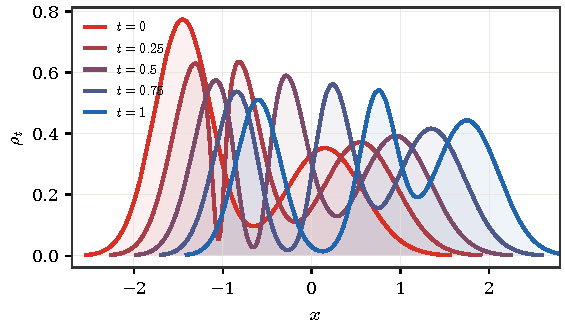
\includegraphics[width=.31\linewidth]{figures/dynamic-benamou-brenier-duality--density.pdf} &
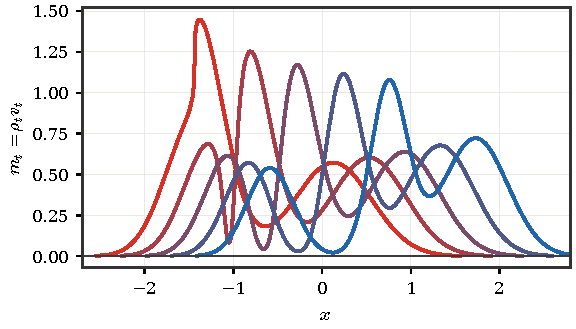
\includegraphics[width=.31\linewidth]{figures/dynamic-benamou-brenier-duality--momentum.pdf} &
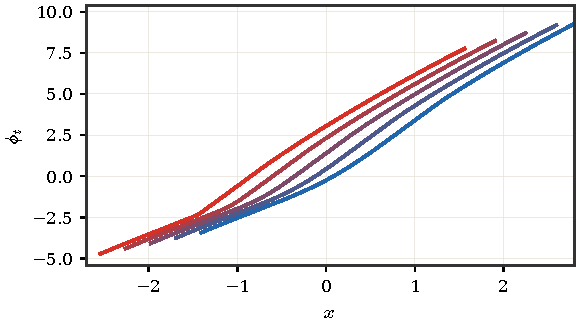
\includegraphics[width=.31\linewidth]{figures/dynamic-benamou-brenier-duality--dual-potential.pdf}
\\[-.1em]
\small density $\rho_t$ &
\small momentum $m_t$ &
\small dual potential $\phi_t$
\end{tabular}
\caption{One-dimensional Benamou--Brenier primal and dual solutions. The endpoints are Gaussian mixtures and the solution is computed from monotone quantile interpolation. The left and middle panels show the primal density and momentum $m_t=\rho_t v_t$. The right panel shows the dual Hamilton--Jacobi potential, normalized up to an additive constant. Along the active transported mass, the notebook checks the primal--dual identities $m_t=\rho_t\partial_x\phi_t/2$ and $\partial_t\phi_t+|\partial_x\phi_t|^2/4=0$.}
\index{Hamilton-Jacobi equation}% strictindex
\index{momentum}% strictindex
\label{fig:dynamic-benamou-brenier-duality}
\end{figure}

\paragraph{Proximal splitting.}
\index{proximal!splitting}% strictindex
\index{Douglas-Rachford!splitting}% strictindex

The convex momentum formulation also explains the original Benamou--Brenier solver. Papadakis, Peyr\'e and Oudet~\cite{FPapPeyOud13} showed that, after discretization, the ALG2 scheme is a Douglas--Rachford splitting, equivalently ADMM on the Fenchel--Rockafellar dual. Suppressing discretization indices, write $U=(\rho,m)$ and introduce the perspective integrand
\[
	J(\rho,m)=
	\begin{cases}
		\norm{m}^2/\rho, & \rho>0,\\
		0, & (\rho,m)=(0,0),\\
		+\infty, & \text{otherwise}.
	\end{cases}
\]
Let
\[
	\mathcal F(U)=\int_0^1\!\int_{\RR^d}J(\rho_t(x),m_t(x))\,\d x\,\d t,
	\qquad
	\mathcal C=\enscond{(\rho,m)}{\partial_t\rho+\diverg m=0,\ \rho_0\d x=\alpha_0,\ \rho_1\d x=\alpha_1},
\]
and let $\mathcal G=\iota_{\mathcal C}$ be the indicator of this affine continuity constraint. The convex Benamou--Brenier problem is therefore
\[
	\min_U\; \mathcal F(U)+\mathcal G(U).
\]
On the resulting Hilbert space of unknowns, or formally for an $L^2$-type product structure, the two proximal operators are
\[
	\prox_{\tau\mathcal F}(\bar U)
	=
	\argmin_U
	\frac12\norm{U-\bar U}_{\mathsf H}^2+\tau\mathcal F(U),
	\qquad
	\prox_{\tau\mathcal G}(\bar U)
	=
	\argmin_{U\in\mathcal C}
	\frac12\norm{U-\bar U}_{\mathsf H}^2 .
\]
For the standard product metric, the first map is local in $(t,x)$: it is the proximal operator of the convex perspective $J$. The second map is the orthogonal projection onto the affine set defined by the divergence equation and endpoint constraints. Douglas--Rachford then alternates these two simple operations:
\[
	\begin{aligned}
		U^{k+1} &= \prox_{\tau\mathcal F}(Z^k),\\
		\widetilde U^{k+1} &= \prox_{\tau\mathcal G}(2U^{k+1}-Z^k),\\
		Z^{k+1} &= Z^k+\widetilde U^{k+1}-U^{k+1}.
	\end{aligned}
\]
Equivalently one may swap the roles of $\mathcal F$ and $\mathcal G$. At convergence, the two shadow sequences $U^k$ and $\widetilde U^k$ agree and give a minimizer of the convex dynamic problem. This viewpoint is useful because it separates the nonlinear but pointwise perspective proximal step from the global but linear projection onto the continuity equation~\cite{FPapPeyOud13,Eckstein1992}.
\index{perspective function}% strictindex
\index{continuity equation}% strictindex
\index{Fenchel-Rockafellar duality}% strictindex
\index{ADMM}% strictindex

\begin{alg}[Douglas--Rachford for dynamic Benamou--Brenier]\label{alg:benamou-brenier-douglas-rachford}
\index{Douglas-Rachford!splitting}% strictindex
\textbf{Input:} Functionals $\mathcal F,\mathcal G=\iota_{\mathcal C}$, proximal parameter $\tau>0$, initial field $Z^0$.

\textbf{Output:} Discrete density-momentum field $U^\star$.

\textbf{For} $k=0,1,\ldots$ \textbf{do}:
\begin{algblock}
\(U^{k+1}=\prox_{\tau\mathcal F}(Z^k).\)

\textbf{Project} reflected point:
\(\widetilde U^{k+1} = \prox_{\tau\mathcal G}(2U^{k+1}-Z^k) = \Proj_{\mathcal C}(2U^{k+1}-Z^k).\)

\textbf{Update}
\(Z^{k+1}=Z^k+\widetilde U^{k+1}-U^{k+1}.\)

\textbf{If} $\norm{U^{k+1}-\widetilde U^{k+1}}\leq\mathrm{tol}$ \textbf{then}:
\begin{algblock}
\textbf{Return} $U^{k+1}$.
\end{algblock}
\end{algblock}
\end{alg}

\begin{figure}[ht]
\centering
\newcommand{\bbgeodesicpanelheight}{.155\linewidth}
\begin{tabular}{@{}cc@{}}

\includegraphics[height=\bbgeodesicpanelheight]{figures/dynamic-benamou-brenier-geodesic--density-sequence.pdf} &
\index{Benamou-Brenier}% strictindex
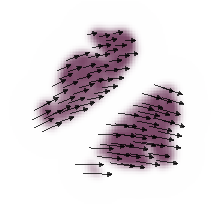
\includegraphics[height=\bbgeodesicpanelheight]{figures/dynamic-benamou-brenier-geodesic--midpoint-velocities.pdf}
\\[-.1em]
\small density sequence &
\small midpoint velocities
\end{tabular}
\caption{Benamou--Brenier geodesic between two sampled silhouettes. A discrete quadratic OT plan between finely subsampled cat and two-disks point clouds induces the McCann interpolation $Z_t=(1-t)X+tY$, which is the Lagrangian realization of the least-action solution. The left panel renders local color images of the smaller-bandwidth kernel-smoothed densities with enough padding to include the full silhouettes. The right panel overlays shortened velocity arrows centered at evenly subsampled midpoint particles $Z_{1/2}$; each displayed arrow runs in data coordinates from a source-side tail to a target-side head along the matched characteristic direction $Y-X$, but is not drawn as the full endpoint segment from $X$ to $Y$.}
\index{McCann interpolation}% strictindex
\index{Benamou-Brenier}% strictindex
\label{fig:dynamic-benamou-brenier-geodesic}
\end{figure}

\begin{rem}[Path-space formulation]\label{rem-bb-path-space}
\index{path-space!formulation}% strictindex
	Let $\Ss=C([0,1];\RR^d)$ be the space of continuous paths endowed with the uniform topology. For $t\in[0,1]$ define the evaluation map
	\[
		P_t:\Ss\to\RR^d,
		\qquad
		P_t(\gamma)=\gamma(t).
	\]
	The Benamou--Brenier cost admits the equivalent formulation
\index{Benamou-Brenier}% strictindex
	\[
		\Wass_2^2(\alpha_0,\alpha_1)
		=
		\inf_{M\in\Pp(\Ss)}
		\enscond{
			\int_{\Ss}\!\int_0^1\norm{\dot\gamma(t)}^2\d t\,\d M(\gamma)
		}{
			(P_0)_\sharp M=\alpha_0,\ (P_1)_\sharp M=\alpha_1
		}.
	\]
	If $\alpha_0$ has a density, the minimizer $M^*$ is unique. Its time marginals reproduce the optimal curve: $\alpha_t=(P_t)_\sharp M^*$ for all $t$. Furthermore, for a.e. $t$, denoting $Q_t(\gamma)=\dot\gamma(t)$ on absolutely continuous paths, the conditional law of the velocity is deterministic:
\index{absolutely continuous path}% strictindex
\index{conditional law}% strictindex
	\[
		(P_t,Q_t)_\sharp M^*(\d x,\d q)
		=
		\alpha_t(\d x)\delta_{v_t^*(x)}(\d q),
	\]
	where $v_t^*$ is the optimal velocity field in the Benamou--Brenier formulation. Hence $M^*$ concentrates on straight-line geodesics and, for a.e. $t$, assigns exactly one direction at $\alpha_t$-a.e. spatial point.
\index{Benamou-Brenier}% strictindex
\index{velocity field}% strictindex
\index{Benamou-Brenier!formulation}% strictindex
\end{rem}

\paragraph{Extensions of the dynamic formulation.}
\index{dynamic!formulation}% strictindex
\label{sec-bb-extensions}

The same variational grammar extends beyond the quadratic Wasserstein distance. One changes either the kinetic exponent, the mobility or the balance equation, while keeping a continuity-type constraint and a convex perspective action.
\index{Wasserstein!distance}% strictindex

\begin{rem}[Generalized Benamou--Brenier distances]\label{rem-generalized-bb}
\index{Benamou-Brenier}% strictindex
\index{Benamou-Brenier!distance}% strictindex
	The dynamic formulation is not specific to $\Wass_2$. For measures with finite $p$-th moments and $p>1$, one has the analogous action formula
\index{dynamic!formulation}% strictindex
	\[
		\Wass_p^p(\alpha_0,\alpha_1)
		=
		\inf_{\substack{\partial_t\alpha_t+\nabla\!\cdot(\alpha_t v_t)=0\\
		\alpha_{t=0}=\alpha_0,\ \alpha_{t=1}=\alpha_1}}
		\int_0^1\!\int_{\RR^d} |v_t(x)|^p\,\d\alpha_t(x)\,\d t.
	\]
	When $\alpha_t=\rho_t\,\d x$ and $m_t=\rho_t v_t$, this becomes the convex perspective action
	\[
		\int_0^1\!\int_{\RR^d}
		\frac{|m_t(x)|^p}{\rho_t(x)^{p-1}}\,\d x\,\d t,
		\qquad
		\partial_t\rho_t+\nabla\!\cdot m_t=0,
	\]
	with the usual convention that the integrand is $0$ if $(\rho,m)=(0,0)$ and $+\infty$ if $\rho=0$ but $m\neq0$.

	A second class of variants changes the mobility of the medium: the quadratic action $|m|^2/\rho$ is replaced by $|m|^2/\theta(\rho)$ for a suitable concave mobility $\theta$. Under appropriate structural assumptions, this produces transport metrics adapted to nonlinear diffusions and finite-volume discretizations~\cite{dolbeault2009new}. On finite graphs and Markov chains, the analogous action uses an edge mobility, often the logarithmic mean of the endpoint densities, and leads to discrete Wasserstein geometries~\cite{Maas2011,MielkeCVPDE}. These extensions keep the same variational grammar as Benamou--Brenier: a continuity-type constraint, an action density, and geodesics obtained by minimizing an integrated kinetic cost.
\index{Benamou-Brenier}% strictindex
\end{rem}

\paragraph{Dynamic unbalanced OT.}
\label{sec-unbalanced-ot}
\index{unbalanced!OT}% strictindex
\index{dynamic!unbalanced OT}% strictindex

Unbalanced dynamic transport is obtained by allowing mass to be created and destroyed along the path. The continuity equation is replaced by a balance equation, and the action penalizes both spatial motion and growth. This dynamic formulation underlies the Hellinger--Kantorovich and Wasserstein--Fisher--Rao metrics~\cite{LieroMielkeSavareShort,2017-chizat-focm}; its equivalence with static entropy-transport and cone formulations is developed in~\cite{LieroMielkeSavareLong,2015-chizat-unbalanced}. A representative quadratic action is
\index{continuity equation}% strictindex
	\[
		\partial_t\rho_t+\nabla\!\cdot m_t=s_t,
		\qquad
		\int_0^1\!\int
		\left(\frac{|m_t|^2}{\rho_t}+\kappa^2\frac{s_t^2}{\rho_t}\right)\d x\,\d t,
	\]
	with the same perspective convention as above. Equivalently, writing $m_t=\rho_t v_t$ and $s_t=\rho_t g_t$, one minimizes $\int_0^1\int(|v_t|^2+\kappa^2 g_t^2)\d\rho_t\d t$ under $\partial_t\rho_t+\nabla\!\cdot(\rho_t v_t)=g_t\rho_t$. The parameter $\kappa$ fixes the relative cost of reaction and transport; changing it rescales the radial/angular balance in the associated cone metric. For measure-valued triples, the action is understood in the lower-semicontinuous perspective sense
	\[
		\mathcal A_\kappa(\rho,m,s)
		\eqdef
		\int
		\left(
			\frac{\norm{\dot m}^2}{\dot\rho}
			+
			\kappa^2\frac{\dot s^2}{\dot\rho}
		\right)\d\lambda,
		\qquad
		(\dot\rho,\dot m,\dot s)
		=
		\left(\frac{\d\rho}{\d\lambda},\frac{\d m}{\d\lambda},\frac{\d s}{\d\lambda}\right),
	\]
	where $\lambda$ dominates $\rho$ and the total variations of $m$ and $s$, and the value is independent of this choice. The convention is $0/0=0$ and $a/0=+\infty$ for $a>0$, so finite action forces both the flux and source to be absolutely continuous with respect to the transported mass.
\index{balance equation}% strictindex
\index{Hellinger-Kantorovich}% strictindex
\index{Wasserstein-Fisher-Rao}% strictindex

\begin{prop}[Static/dynamic equivalence for unbalanced OT]\label{prop-static-dynamic-unbalanced}
\index{static-dynamic equivalence}% strictindex
\index{unbalanced!OT}% strictindex
		Fix the action above and let $\CW_\kappa$ be the cone value of Theorem~\ref{thm-cone-unbalanced-ot} with the cone metric normalized to the same growth scale $\kappa$. For nonnegative finite measures $\alpha_0,\alpha_1$ on $\RR^d$, the dynamic value
	\begin{equation}\label{eq-dynamic-unbalanced-ot}
		\WFR_\kappa^2(\alpha_0,\alpha_1)
		\eqdef
		\inf_{\substack{\partial_t\rho_t+\nabla\cdot m_t=s_t\\
		\rho_0=\alpha_0,\ \rho_1=\alpha_1}}
		\int_0^1
		\mathcal A_\kappa(\rho_t,m_t,s_t)\,\d t
	\end{equation}
		equals the static cone formulation $\CW_\kappa(\alpha_0,\alpha_1)$. Hence the static unbalanced problem and the balance-equation least-action problem define the same geodesic distance.
\end{prop}

\begin{proof}
	The cone construction turns variation of mass into radial motion and spatial transport into angular motion on $\mathfrak C[\RR^d]$. Applying the Benamou--Brenier theorem on the cone to the lifted endpoint measures gives a dynamic least-action problem on $\mathfrak C[\RR^d]$ whose static value is the cone value $\CW_\kappa$ of Theorem~\ref{thm-cone-unbalanced-ot}. This is the standard static/dynamic identification for the Hellinger--Kantorovich and Wasserstein--Fisher--Rao metrics~\cite{LieroMielkeSavareShort,LieroMielkeSavareLong,2017-chizat-focm,2015-chizat-unbalanced}.
\index{cone!lifting}% strictindex
\index{Benamou-Brenier}% strictindex

	Projecting a cone curve back to the base space with the weight $r^2$ produces a measure curve $\rho_t$, a spatial flux $m_t$ and a source term $s_t$ satisfying the balance equation. With the matching normalization of the cone metric, the cone kinetic energy decomposes exactly into the perspective action $\mathcal A_\kappa$ in~\eqref{eq-dynamic-unbalanced-ot}. Conversely, any finite-action triple $(\rho_t,m_t,s_t)$ can be lifted to a cone curve whose radial velocity realizes the growth term and whose spatial velocity realizes the transport term, with the same action after relaxation. The two infima are therefore equal; lower semicontinuity gives the general finite-measure statement from the smooth positive case.
\index{lower semicontinuity}% strictindex
\end{proof}

\begin{figure}[H]
\centering
\setlength{\tabcolsep}{1pt}
\begin{tabular}{@{}rccccc@{}}
& \small $t=0$ & \small $t=.25$ & \small $t=.5$ & \small $t=.75$ & \small $t=1$ \\
\small balanced &
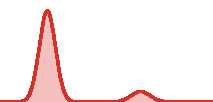
\includegraphics[width=.165\linewidth]{figures/dynamic-unbalanced-geodesic--balanced-t000.pdf} &
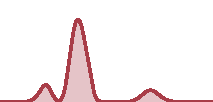
\includegraphics[width=.165\linewidth]{figures/dynamic-unbalanced-geodesic--balanced-t025.pdf} &
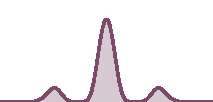
\includegraphics[width=.165\linewidth]{figures/dynamic-unbalanced-geodesic--balanced-t050.pdf} &
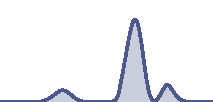
\includegraphics[width=.165\linewidth]{figures/dynamic-unbalanced-geodesic--balanced-t075.pdf} &
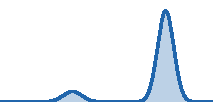
\includegraphics[width=.165\linewidth]{figures/dynamic-unbalanced-geodesic--balanced-t100.pdf} \\
\small unbalanced &
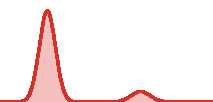
\includegraphics[width=.165\linewidth]{figures/dynamic-unbalanced-geodesic--unbalanced-t000.pdf} &
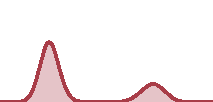
\includegraphics[width=.165\linewidth]{figures/dynamic-unbalanced-geodesic--unbalanced-t025.pdf} &
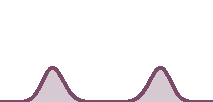
\includegraphics[width=.165\linewidth]{figures/dynamic-unbalanced-geodesic--unbalanced-t050.pdf} &
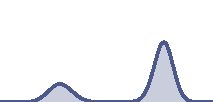
\includegraphics[width=.165\linewidth]{figures/dynamic-unbalanced-geodesic--unbalanced-t075.pdf} &
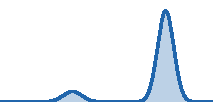
\includegraphics[width=.165\linewidth]{figures/dynamic-unbalanced-geodesic--unbalanced-t100.pdf}
\end{tabular}
\caption{Balanced and unbalanced Sinkhorn-barycenter interpolations between two one-dimensional Gaussian mixtures with swapped modal masses. The balanced row conserves total mass, so excess mass from the dominant left mode must move along the line toward the dominant right target mode, producing transient mass in the middle. The unbalanced row uses KL-relaxed marginal constraints; mass can be attenuated near overrepresented modes and recreated near underrepresented modes, giving a reaction--transport interpolation closer to the Wasserstein--Fisher--Rao intuition.}
\index{Sinkhorn!barycenter}% strictindex
\index{unbalanced!barycenter}% strictindex
\label{fig:dynamic-unbalanced-geodesic}
\end{figure}
